\documentclass[a4paper]{article}

% Packages
\usepackage[utf8]{inputenc}
\usepackage[margin=1in]{geometry}
\usepackage{amsmath}
\usepackage{booktabs}
\usepackage{caption}
\usepackage{enumitem}
\usepackage{float}
\usepackage{graphicx}
\usepackage{hyperref}
\usepackage{makecell}
\usepackage{microtype}
\usepackage{tabularx}
\usepackage{tikz}
\usepackage{titlesec}

% Title
\title{Scalable Rendering Graphics and Game Engine}

\author{
    \Large Peter Yaacoub \\[1ex]
    \normalsize\textit{Universitat Politècnica de Catalunya (UPC)} \\[3ex]
}

\date{\vspace{1ex} May 2026}

% Document
\begin{document}
\maketitle

\section{Session 1: Base Engine and Museum Floorplan}

The foundational session establishes the core rendering infrastructure and the museum environment pipeline. It adds the first complete path from a map file to a rendered scene, together with the initial navigation and fullscreen controls.

\subsection{Implemented Features}
\begin{itemize}[noitemsep]
    \item \textbf{Model Management:} Extends the engine to support PLY asset loading for high-fidelity meshes, while dynamically generating base render primitives (cubes) in memory to minimize footprint.
    \item \textbf{Procedural Museum Generation:} Parses 2D tile maps into 3D world space. Floors and ceilings are instantiated on open cells, while wall segments are generated based on adjacent open-space detection.
    \item \textbf{Scene Graph Assembly:} Unifies the procedural layout and loaded assets into a cohesive environment by spawning 3D models from map descriptions and applying per-object spatial transforms.
\end{itemize}

\begin{figure}[H]
    \centering
    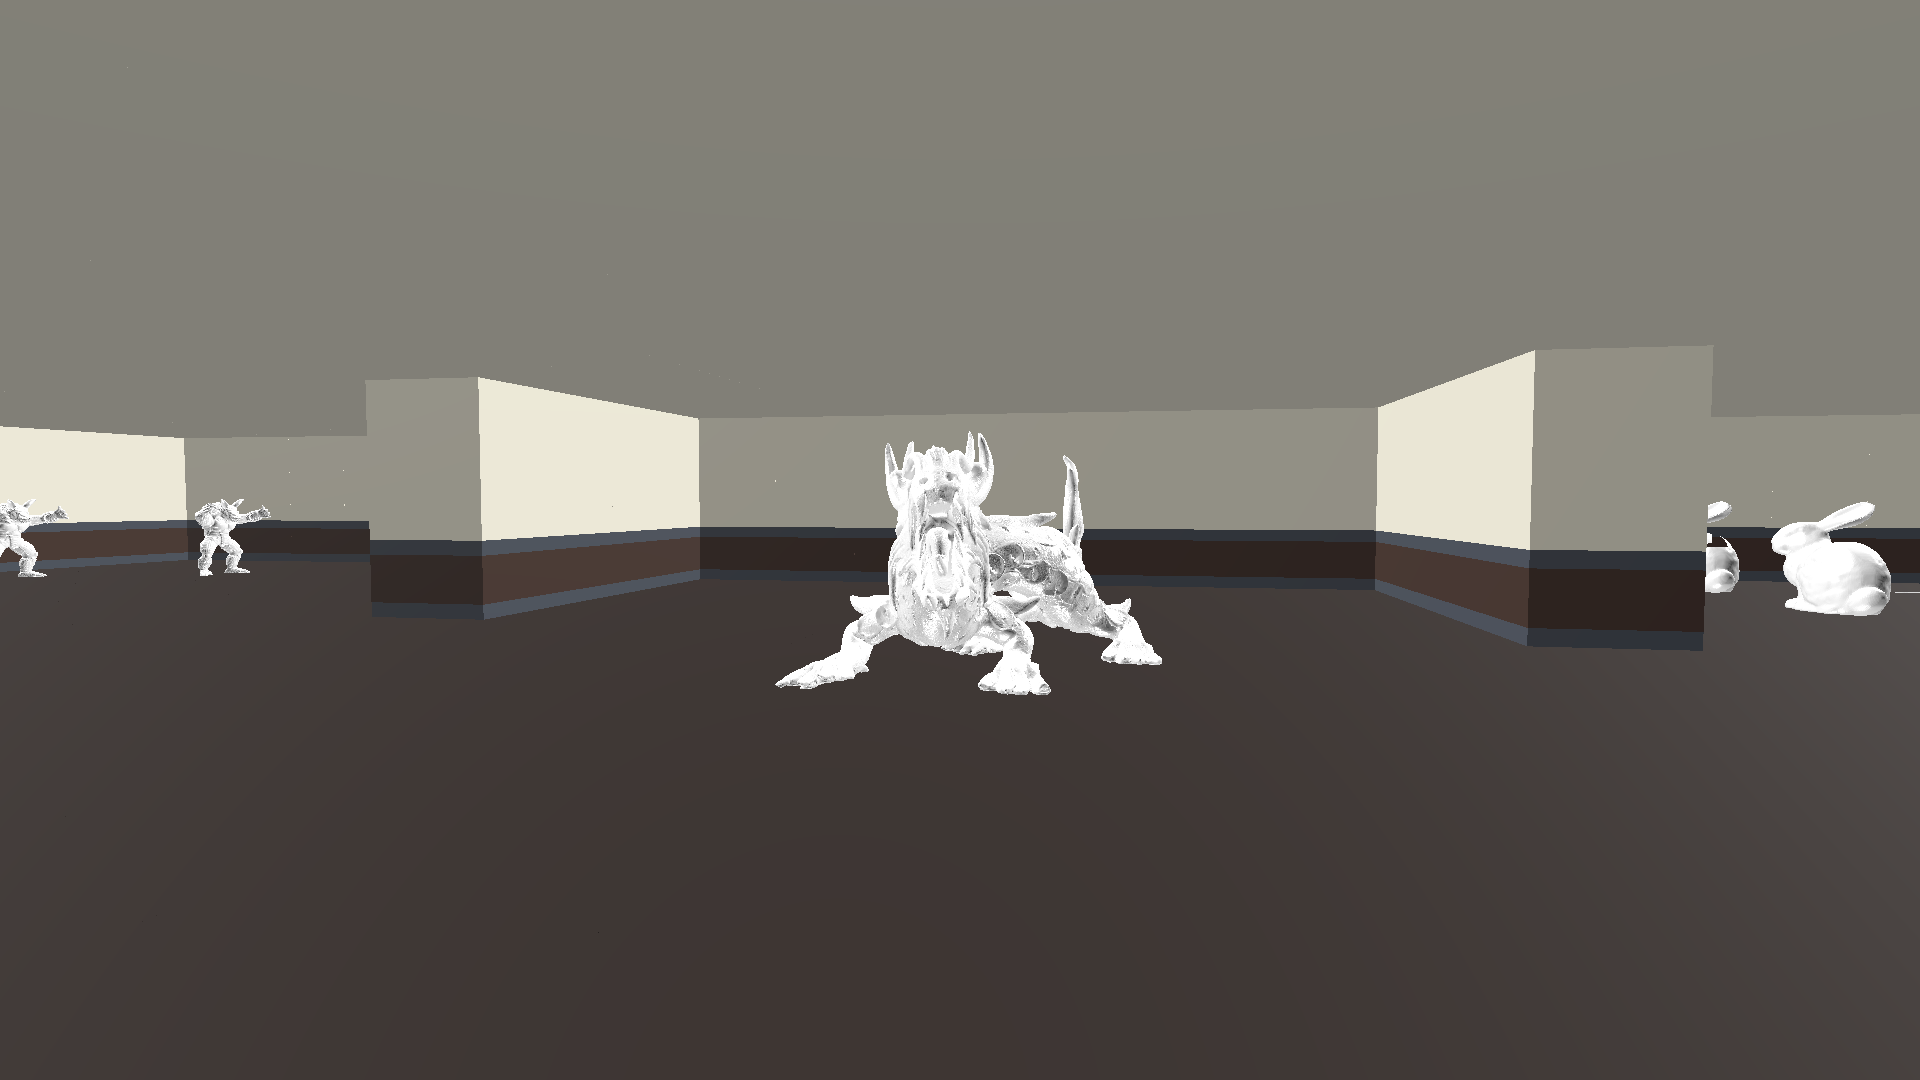
\includegraphics[width=0.8\textwidth]{images/lab1.png}
    \caption{Rendered museum environment showing walls, empty cells, and 3D models.}
\end{figure}

\newpage
\section{Session 2: Mesh Simplification and Levels of Detail}

This session introduces the first simplification pipeline for high-polygon models. The implementation clusters vertices on a regular 3D grid, rebuilds the geometry from cluster representatives, and caches the generated LOD meshes on disk.

\subsection{Implemented Features}
\begin{itemize}[noitemsep]
    \item \textbf{Spatial Vertex Clustering:} Simplifies complex meshes by clustering vertices on a regular 3D grid, using a sparse hash map keyed by voxel coordinates to minimize memory overhead.
    \item \textbf{Cluster Representatives:} Computes the optimal representative for each cell by averaging the spatial positions and color data of all intersecting vertices.
    \item \textbf{Topology Reconstruction:} Rebuilds mesh geometry by reassigning original triangles to the new representative vertices, including automatic detection and removal of degenerate triangles.
    \item \textbf{Progressive LOD Generation:} Creates one of four Level of Detail (LOD) variants from a single source mesh to provide a coarser target resolution.
    \item \textbf{Disk-Based LOD Caching:} Serializes simplified meshes (\_LOD0 to \_LOD3) to disk, allowing subsequent engine runs to bypass the simplification process and reduce load times.
\end{itemize}

\begin{figure}[H]
    \centering
    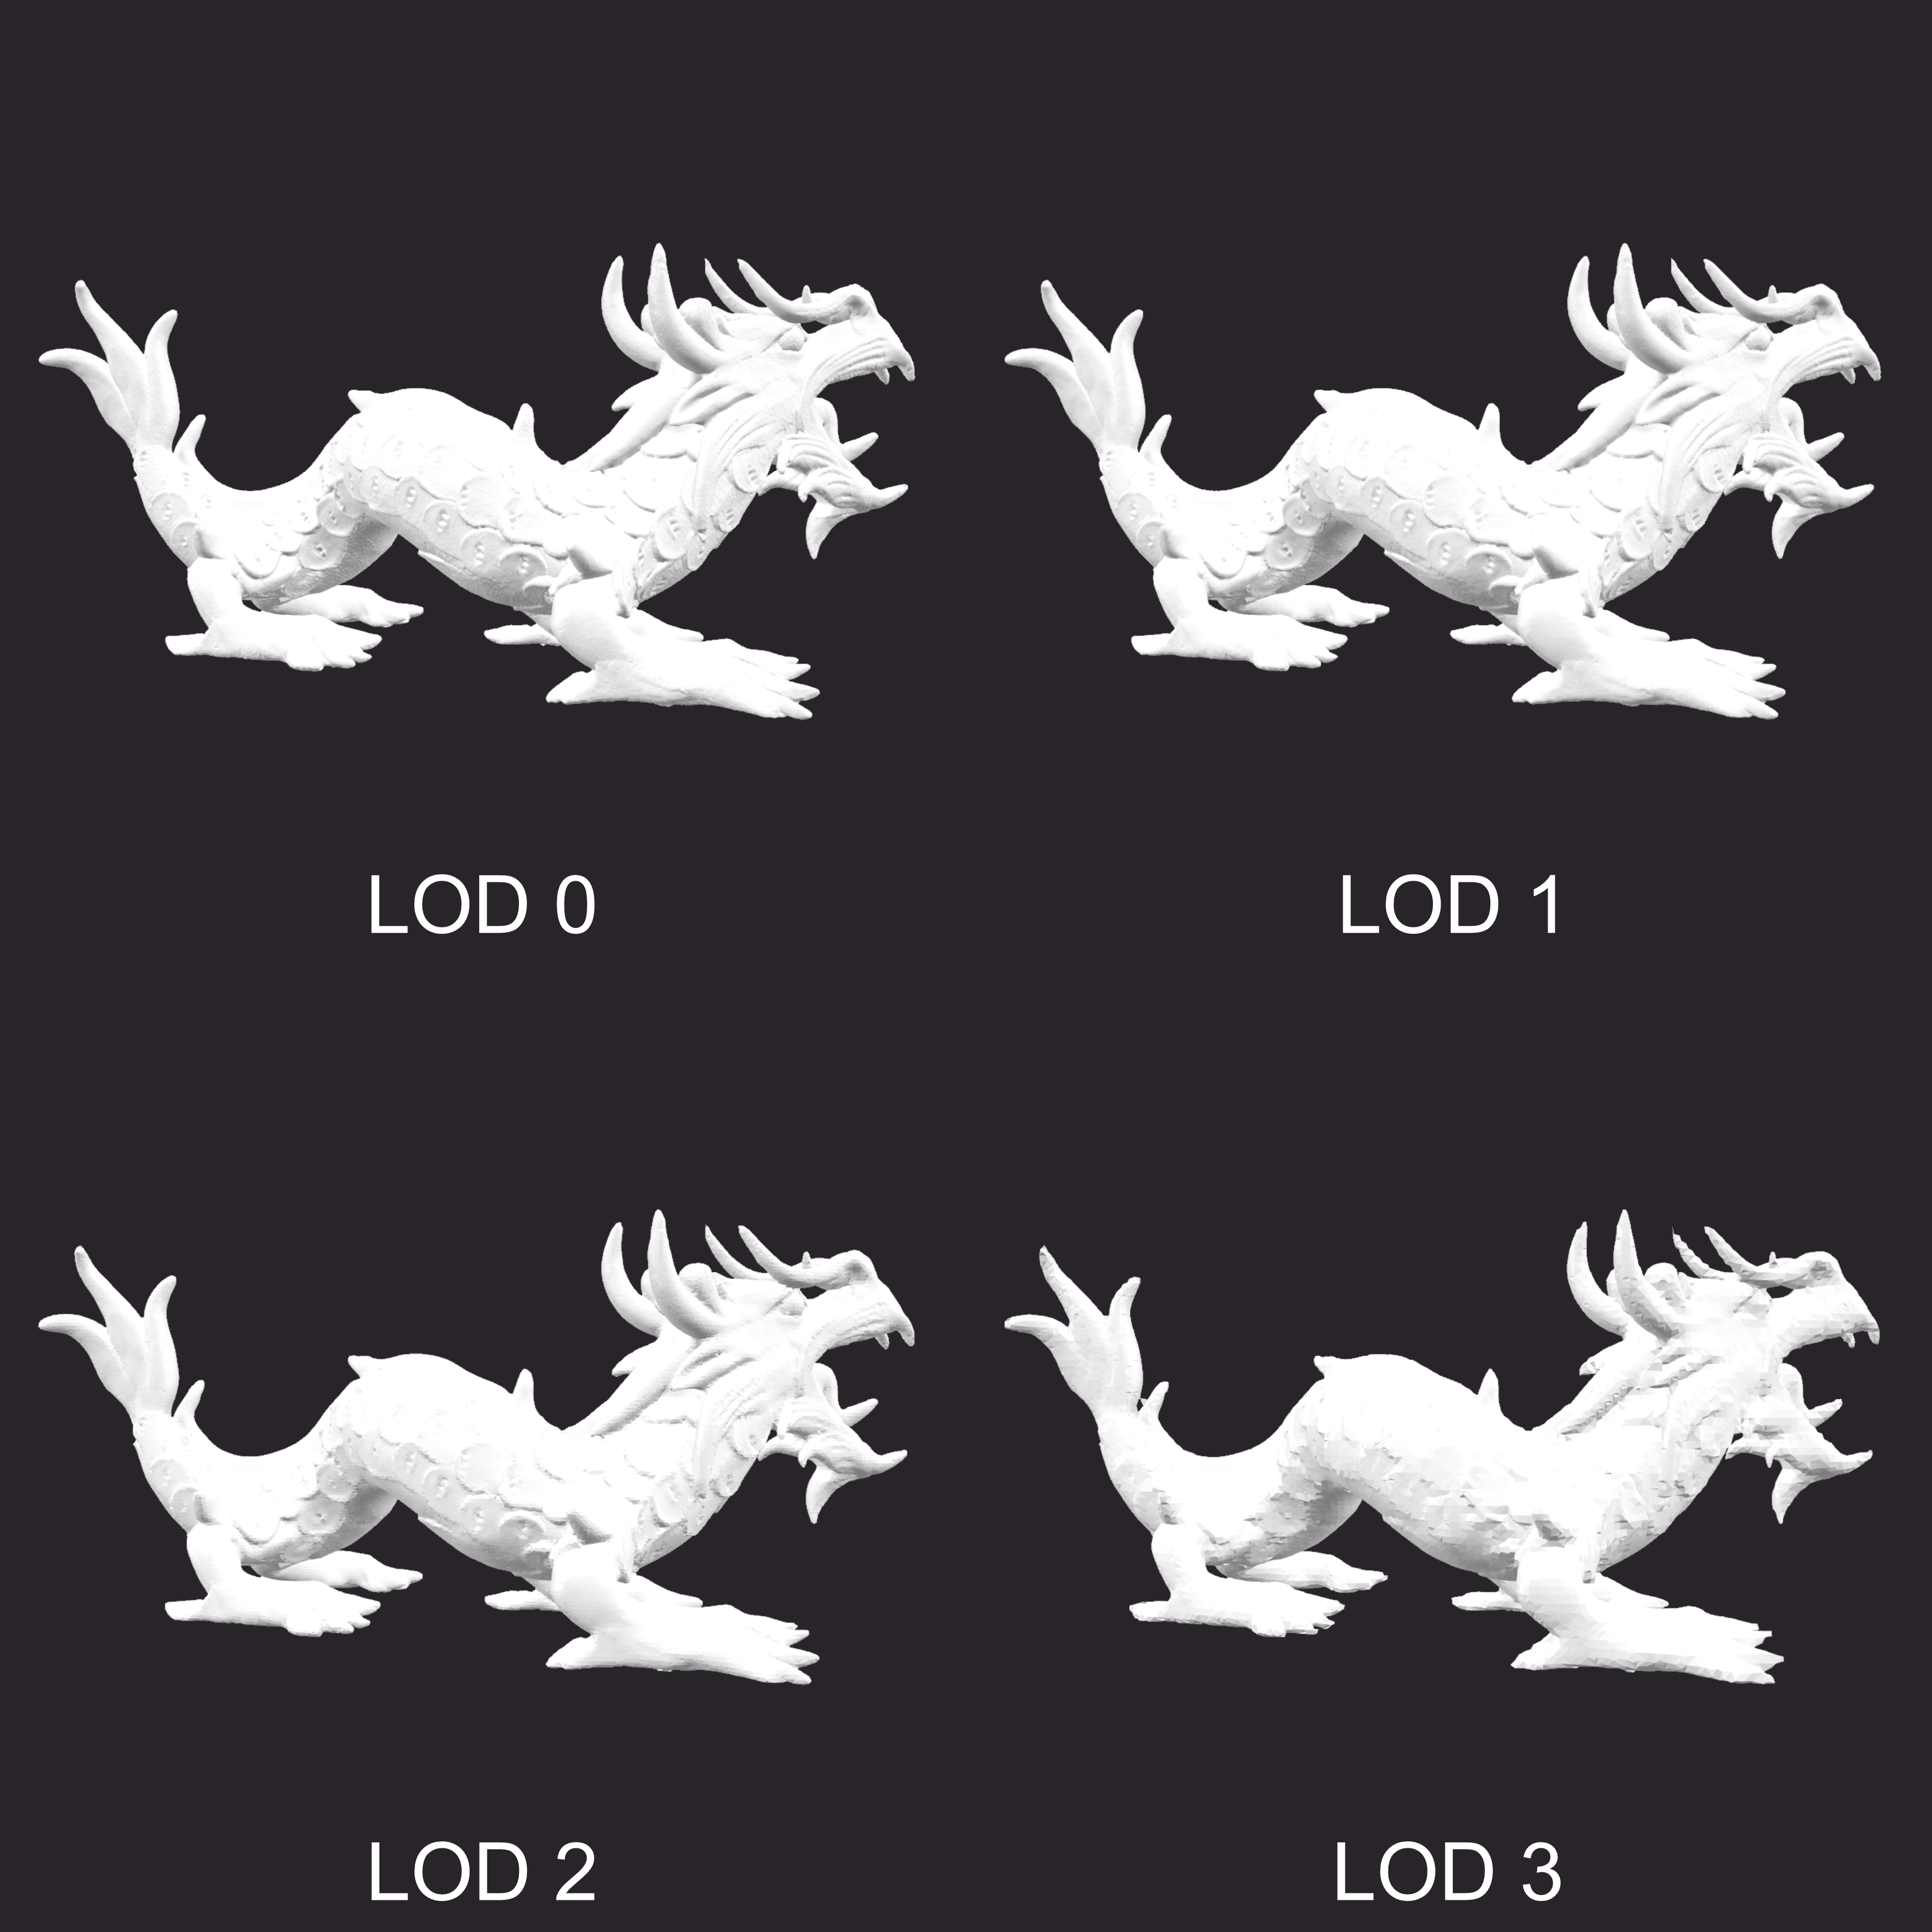
\includegraphics[width=0.8\textwidth]{images/lab2.png}
    \caption{Different Levels of Detail (LODs) generated via vertex clustering.}
\end{figure}

\newpage
\section{Session 3: Quadric Error Metrics (QEM)}

Session 3 replaces the average cluster representative with a Quadric Error Metrics solver, which gives the simplified model a much better geometric fit. The new representative is found by solving the quadric system per occupied grid cell.

\subsection{Implemented Features}
\begin{itemize}[noitemsep]
    \item \textbf{Quadric Matrix Accumulation:} Constructs per-cell quadric matrices derived from the planes of all triangles intersecting a given spatial grid cell.
    \item \textbf{Cell-Centered Error Modeling:} Formulates a cell-centered error metric by expressing each plane relative to the cell center, ensuring accurate geometry reconstruction from the local quadric solution.
    \item \textbf{Robust SVD Solving:} Integrates Eigen::JacobiSVD to compute the pseudo-inverse of the quadric system, providing a mathematically stable solution for rank-deficient and underdetermined cases.
    \item \textbf{Quadric-Optimal Representatives:} Replaces average-vertex clustering with quadric-optimal vertex positioning, significantly improving the geometric fit and silhouette retention of the simplified models.
\end{itemize}

\section{Session 4: Preservation of Thin Features}

To avoid collapsing thin geometry into a single cell, this session adds normal-aware clustering on top of the QEM pipeline. The same spatial cell can now be split into several sub-clusters depending on the orientation of the local surface normals.

\subsection{Implemented Features}
\begin{itemize}[noitemsep]
    \item \textbf{Per-Vertex Normal Accumulation:} Accumulates triangle normals per-vertex to accurately classify the dominant orientation of local surface geometry.
    \item \textbf{Normal Quantization:} Subdivides spatial grid cells into eight distinct sub-cells based on the sign of the X, Y, and Z normal components, preventing opposite-facing surfaces from incorrectly collapsing into each other.
    \item \textbf{Normal-Aware QEM Clustering:} Enhances the QEM simplification pipeline by integrating the normal quantization bucket into the spatial clustering key, ensuring thin features and distinct orientations maintain separate representatives.
\end{itemize}

\begin{figure}[H]
    \centering
    \includegraphics[width=0.8\textwidth]{images/lab4.png}
    \caption{Improved structural preservation of thin features using normal quantization.}
\end{figure}

\newpage
\section{Session 5: Time-Critical Rendering}

This session adds the runtime LOD selector that keeps rendering within a triangle budget. The scene now evaluates which objects deserve more detail, orders upgrades by benefit per cost, and applies the best choices each frame.

\subsection{Implemented Features}
\begin{itemize}[noitemsep]
    \item \textbf{Dynamic Triangle Budgeting:} Calculates real-time frame budgets based on target frame rates and estimated machine throughput, reserving a fixed baseline budget for non-LOD geometry.
    \item \textbf{Cost-Benefit LOD Ranking:} Evaluates available LOD upgrades and sorts them by a ΔBenefit/ΔCost ratio to prioritize the most visually impactful geometric improvements each frame.
    \item \textbf{Distance-Aware Heuristics:} Uses camera distance and object bounding-box diagonals to mathematically estimate the visual benefit of upgrading an object's LOD.
    \item \textbf{Runtime LOD Selection:} Initializes all assets at their coarsest LOD and progressively upgrades them within the active frame until the hardware triangle budget is exhausted.
    \item \textbf{Interactive Debug Visuals:} Provides a runtime debugging mode (toggled via F2) that tints rendered objects based on their active LOD level to visually validate the optimization logic.
\end{itemize}

\begin{figure}[H]
    \centering
    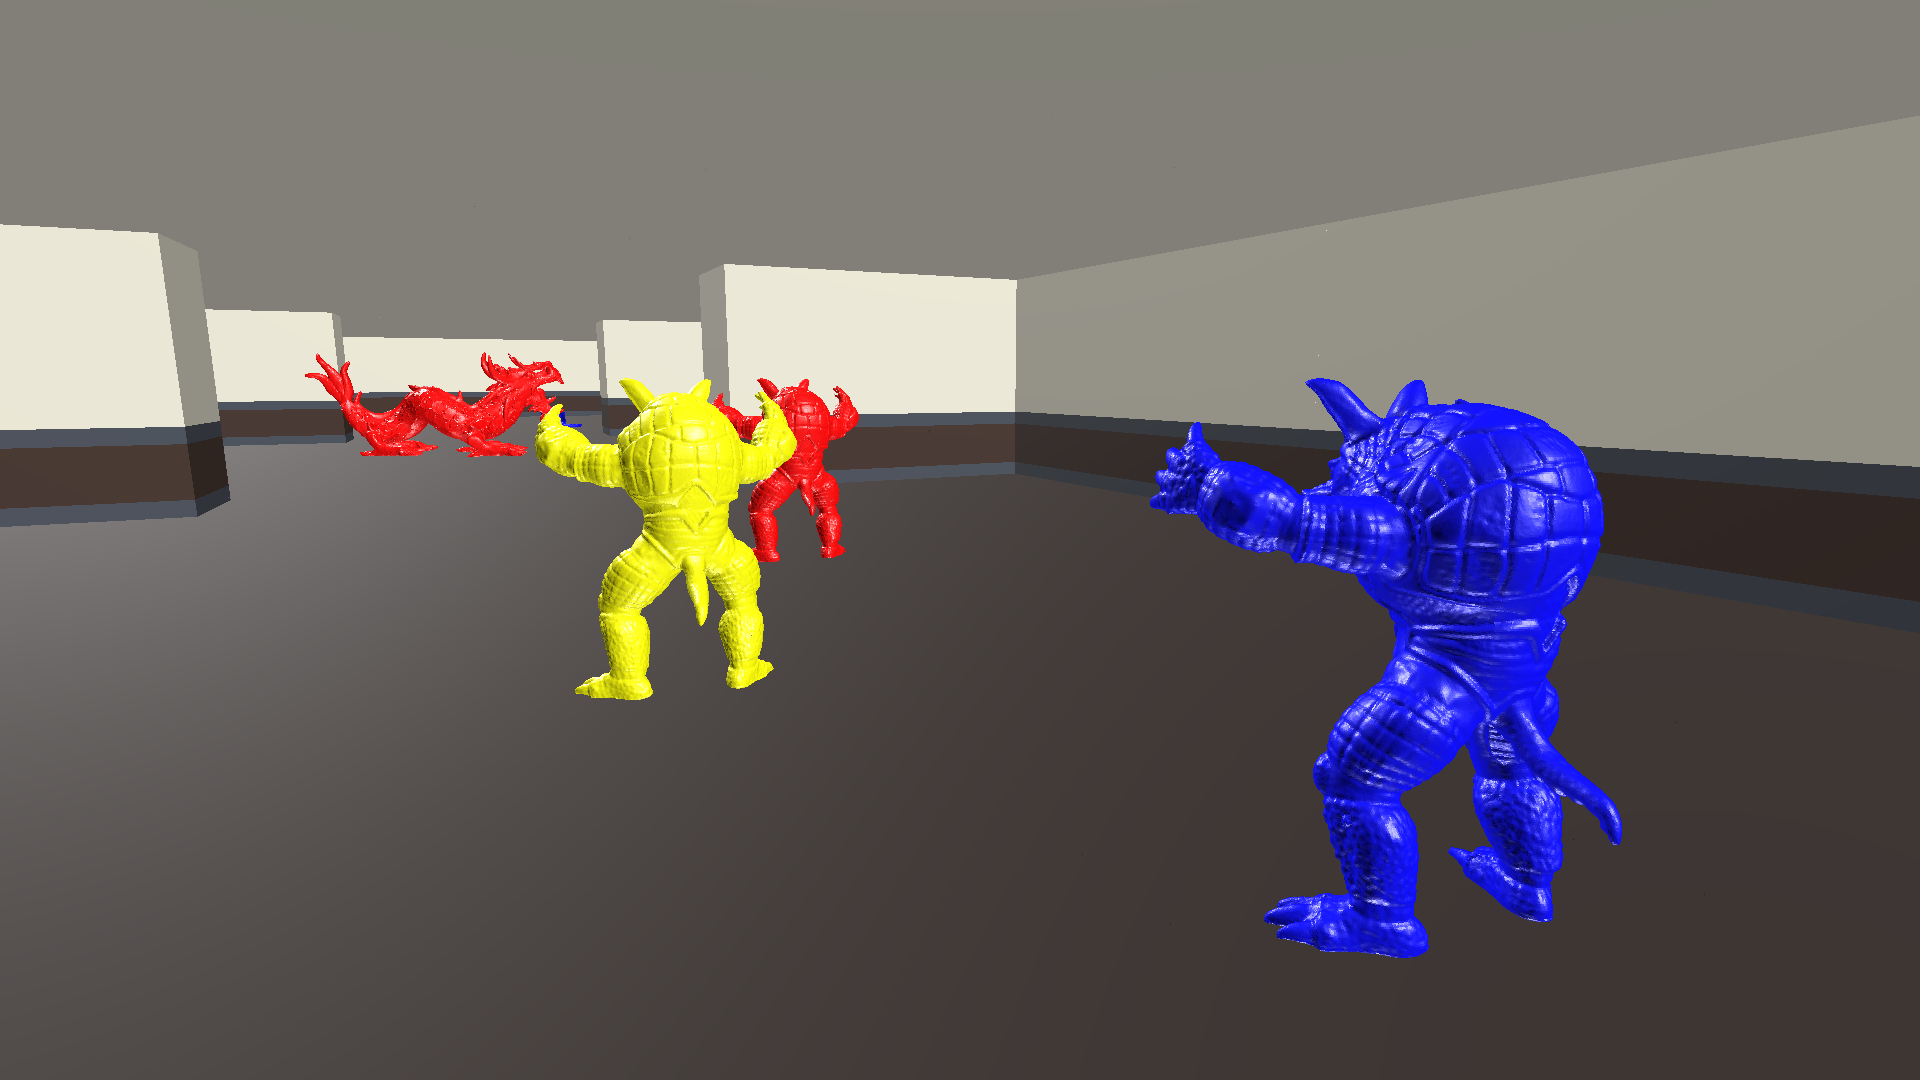
\includegraphics[width=0.8\textwidth]{images/lab5.png}
    \caption{Time-critical rendering adapting LOD dynamically, visualized using LOD coloring.}
\end{figure}

\section{Session 6: Hysteresis Transition}

To eliminate LOD popping and oscillation, this session adds a frame-based hysteresis system. LOD changes are no longer applied immediately; instead, each object must wait for a cooldown period before another transition can occur.

\subsection{Implemented Features}
\begin{itemize}[noitemsep]
    \item \textbf{Frame-Based Cooldowns:} Introduces a waitFrames counter for all LOD-enabled objects to enforce a minimum lifespan for current LOD states, mitigating visual popping.
    \item \textbf{Hysteresis Window Lockout:} Enforces a two-second lockout period following any LOD transition to prevent rapid oscillation when objects hover near a transition threshold.
    \item \textbf{Update Loop Integration:} Embeds the hysteresis countdown directly into the main update loop, ensuring cooldowns are processed seamlessly before the LOD optimizer evaluates the scene.
\end{itemize}

\newpage
\section{Session 7: Cell-to-Cell Visibility Precomputation}

The final session completes the optimization pipeline with offline visibility precomputation and runtime occlusion culling. A separate console tool generates the visibility table, and the renderer uses that table to skip objects that are not visible from the current cell.

\subsection{Implemented Features}
\begin{itemize}[noitemsep]
    \item \textbf{Standalone Visibility Precomputer:} Provides a dedicated, non-OpenGL console utility to ingest map data, sample visibility, and export optimized precomputed data (visibility.txt).
    \item \textbf{Robust Ray Traversal:} Utilizes the Supercover Bresenham algorithm to accurately trace cells crossed by sampled rays, generating a highly conservative visibility map.
    \item \textbf{Visibility Dilation:} Expands visible cells into neighboring boundaries to reduce occlusion popping and improve stability during camera movement near cell edges.
    \item \textbf{Real-Time Occlusion Culling:} Integrates the precomputed visibility grid into the runtime renderer, using the camera's spatial XZ cell to cull non-visible objects and drastically reduce draw calls.
    \item \textbf{Interactive Debug Camera:} Features a togglable bird's-eye debug view (F3) that locks player movement to allow for real-time visual verification of the occlusion culling pipeline.
\end{itemize}

\begin{figure}[H]
    \centering
    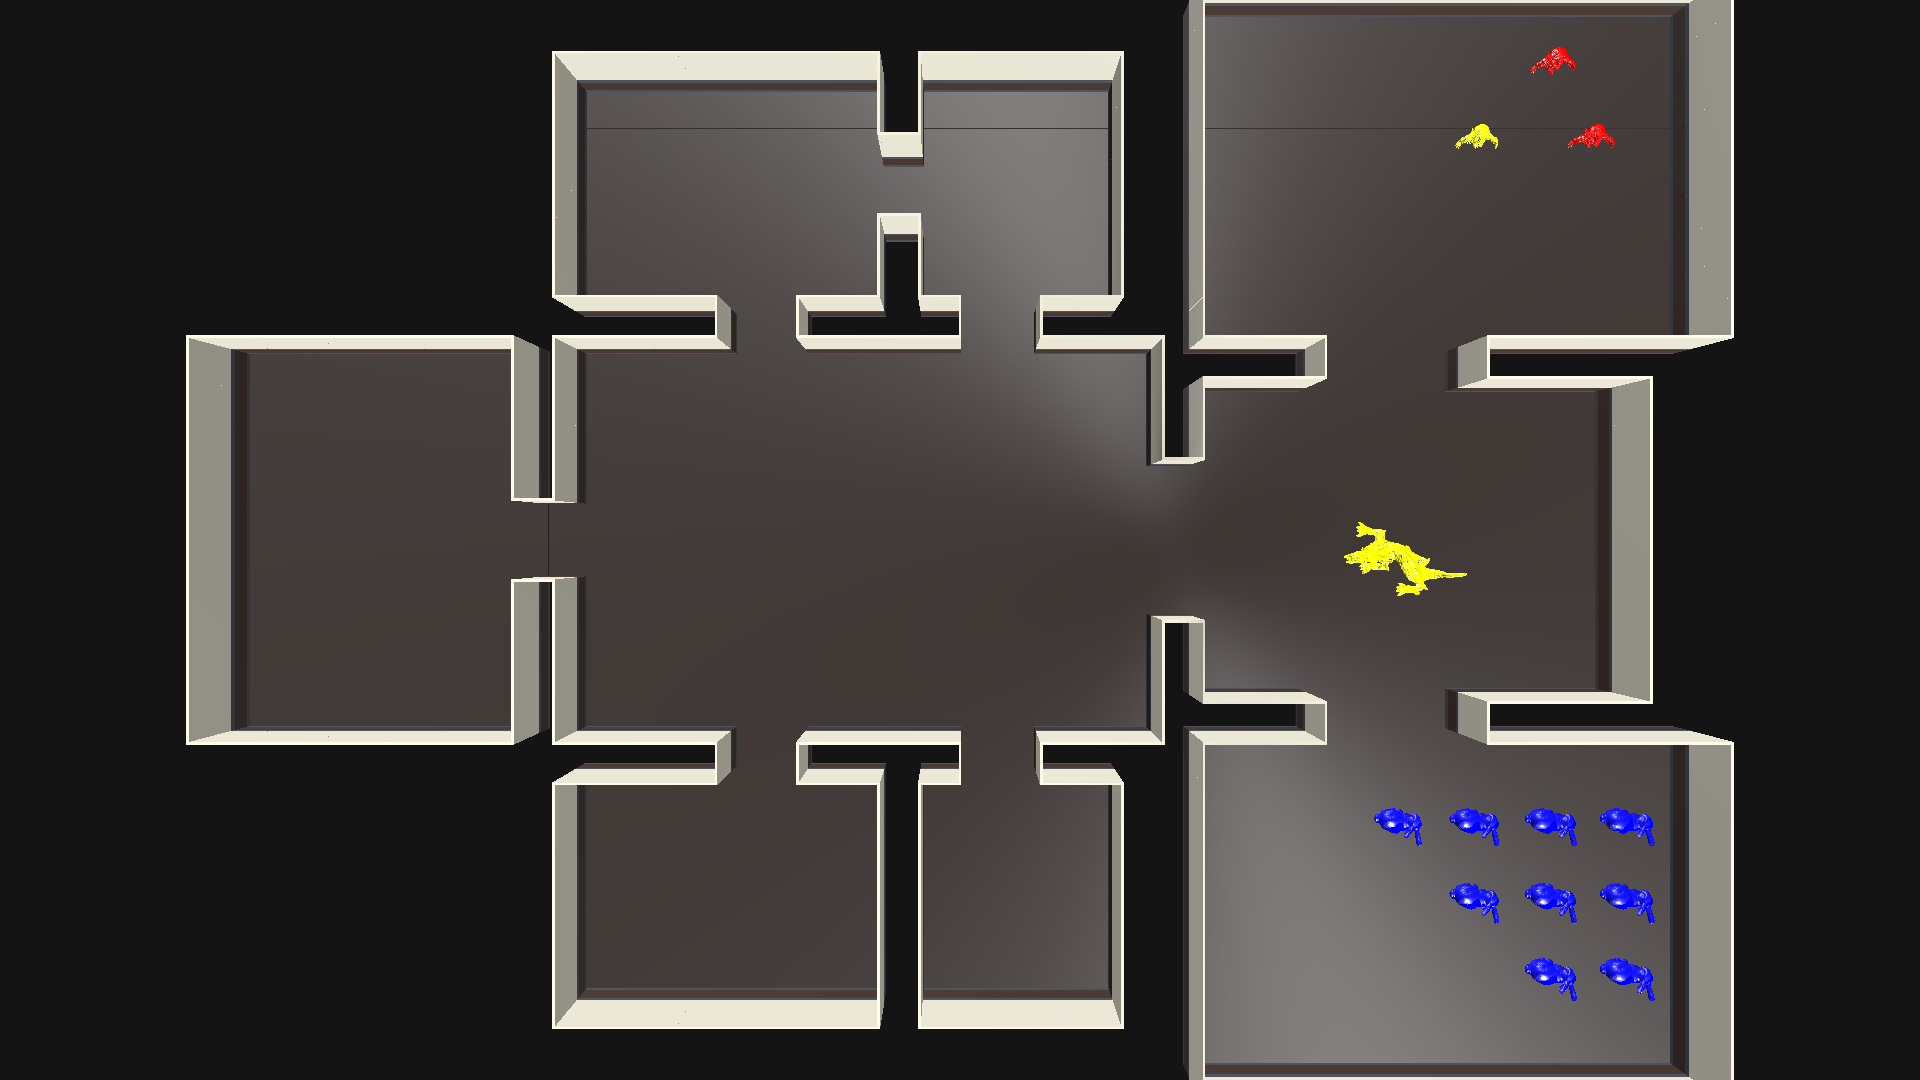
\includegraphics[width=0.8\textwidth]{images/lab7.png}
    \caption{Reduced draw calls resulting from cell-to-cell visibility precomputations.}
\end{figure}

\end{document}